% Options for packages loaded elsewhere
\PassOptionsToPackage{unicode}{hyperref}
\PassOptionsToPackage{hyphens}{url}
%
\documentclass[
]{book}
\usepackage{amsmath,amssymb}
\usepackage{iftex}
\ifPDFTeX
  \usepackage[T1]{fontenc}
  \usepackage[utf8]{inputenc}
  \usepackage{textcomp} % provide euro and other symbols
\else % if luatex or xetex
  \usepackage{unicode-math} % this also loads fontspec
  \defaultfontfeatures{Scale=MatchLowercase}
  \defaultfontfeatures[\rmfamily]{Ligatures=TeX,Scale=1}
\fi
\usepackage{lmodern}
\ifPDFTeX\else
  % xetex/luatex font selection
\fi
% Use upquote if available, for straight quotes in verbatim environments
\IfFileExists{upquote.sty}{\usepackage{upquote}}{}
\IfFileExists{microtype.sty}{% use microtype if available
  \usepackage[]{microtype}
  \UseMicrotypeSet[protrusion]{basicmath} % disable protrusion for tt fonts
}{}
\makeatletter
\@ifundefined{KOMAClassName}{% if non-KOMA class
  \IfFileExists{parskip.sty}{%
    \usepackage{parskip}
  }{% else
    \setlength{\parindent}{0pt}
    \setlength{\parskip}{6pt plus 2pt minus 1pt}}
}{% if KOMA class
  \KOMAoptions{parskip=half}}
\makeatother
\usepackage{xcolor}
\usepackage{color}
\usepackage{fancyvrb}
\newcommand{\VerbBar}{|}
\newcommand{\VERB}{\Verb[commandchars=\\\{\}]}
\DefineVerbatimEnvironment{Highlighting}{Verbatim}{commandchars=\\\{\}}
% Add ',fontsize=\small' for more characters per line
\usepackage{framed}
\definecolor{shadecolor}{RGB}{248,248,248}
\newenvironment{Shaded}{\begin{snugshade}}{\end{snugshade}}
\newcommand{\AlertTok}[1]{\textcolor[rgb]{0.94,0.16,0.16}{#1}}
\newcommand{\AnnotationTok}[1]{\textcolor[rgb]{0.56,0.35,0.01}{\textbf{\textit{#1}}}}
\newcommand{\AttributeTok}[1]{\textcolor[rgb]{0.13,0.29,0.53}{#1}}
\newcommand{\BaseNTok}[1]{\textcolor[rgb]{0.00,0.00,0.81}{#1}}
\newcommand{\BuiltInTok}[1]{#1}
\newcommand{\CharTok}[1]{\textcolor[rgb]{0.31,0.60,0.02}{#1}}
\newcommand{\CommentTok}[1]{\textcolor[rgb]{0.56,0.35,0.01}{\textit{#1}}}
\newcommand{\CommentVarTok}[1]{\textcolor[rgb]{0.56,0.35,0.01}{\textbf{\textit{#1}}}}
\newcommand{\ConstantTok}[1]{\textcolor[rgb]{0.56,0.35,0.01}{#1}}
\newcommand{\ControlFlowTok}[1]{\textcolor[rgb]{0.13,0.29,0.53}{\textbf{#1}}}
\newcommand{\DataTypeTok}[1]{\textcolor[rgb]{0.13,0.29,0.53}{#1}}
\newcommand{\DecValTok}[1]{\textcolor[rgb]{0.00,0.00,0.81}{#1}}
\newcommand{\DocumentationTok}[1]{\textcolor[rgb]{0.56,0.35,0.01}{\textbf{\textit{#1}}}}
\newcommand{\ErrorTok}[1]{\textcolor[rgb]{0.64,0.00,0.00}{\textbf{#1}}}
\newcommand{\ExtensionTok}[1]{#1}
\newcommand{\FloatTok}[1]{\textcolor[rgb]{0.00,0.00,0.81}{#1}}
\newcommand{\FunctionTok}[1]{\textcolor[rgb]{0.13,0.29,0.53}{\textbf{#1}}}
\newcommand{\ImportTok}[1]{#1}
\newcommand{\InformationTok}[1]{\textcolor[rgb]{0.56,0.35,0.01}{\textbf{\textit{#1}}}}
\newcommand{\KeywordTok}[1]{\textcolor[rgb]{0.13,0.29,0.53}{\textbf{#1}}}
\newcommand{\NormalTok}[1]{#1}
\newcommand{\OperatorTok}[1]{\textcolor[rgb]{0.81,0.36,0.00}{\textbf{#1}}}
\newcommand{\OtherTok}[1]{\textcolor[rgb]{0.56,0.35,0.01}{#1}}
\newcommand{\PreprocessorTok}[1]{\textcolor[rgb]{0.56,0.35,0.01}{\textit{#1}}}
\newcommand{\RegionMarkerTok}[1]{#1}
\newcommand{\SpecialCharTok}[1]{\textcolor[rgb]{0.81,0.36,0.00}{\textbf{#1}}}
\newcommand{\SpecialStringTok}[1]{\textcolor[rgb]{0.31,0.60,0.02}{#1}}
\newcommand{\StringTok}[1]{\textcolor[rgb]{0.31,0.60,0.02}{#1}}
\newcommand{\VariableTok}[1]{\textcolor[rgb]{0.00,0.00,0.00}{#1}}
\newcommand{\VerbatimStringTok}[1]{\textcolor[rgb]{0.31,0.60,0.02}{#1}}
\newcommand{\WarningTok}[1]{\textcolor[rgb]{0.56,0.35,0.01}{\textbf{\textit{#1}}}}
\usepackage{longtable,booktabs,array}
\usepackage{calc} % for calculating minipage widths
% Correct order of tables after \paragraph or \subparagraph
\usepackage{etoolbox}
\makeatletter
\patchcmd\longtable{\par}{\if@noskipsec\mbox{}\fi\par}{}{}
\makeatother
% Allow footnotes in longtable head/foot
\IfFileExists{footnotehyper.sty}{\usepackage{footnotehyper}}{\usepackage{footnote}}
\makesavenoteenv{longtable}
\usepackage{graphicx}
\makeatletter
\def\maxwidth{\ifdim\Gin@nat@width>\linewidth\linewidth\else\Gin@nat@width\fi}
\def\maxheight{\ifdim\Gin@nat@height>\textheight\textheight\else\Gin@nat@height\fi}
\makeatother
% Scale images if necessary, so that they will not overflow the page
% margins by default, and it is still possible to overwrite the defaults
% using explicit options in \includegraphics[width, height, ...]{}
\setkeys{Gin}{width=\maxwidth,height=\maxheight,keepaspectratio}
% Set default figure placement to htbp
\makeatletter
\def\fps@figure{htbp}
\makeatother
\setlength{\emergencystretch}{3em} % prevent overfull lines
\providecommand{\tightlist}{%
  \setlength{\itemsep}{0pt}\setlength{\parskip}{0pt}}
\setcounter{secnumdepth}{5}
\usepackage{booktabs}
\ifLuaTeX
  \usepackage{selnolig}  % disable illegal ligatures
\fi
\usepackage[]{natbib}
\bibliographystyle{apalike}
\IfFileExists{bookmark.sty}{\usepackage{bookmark}}{\usepackage{hyperref}}
\IfFileExists{xurl.sty}{\usepackage{xurl}}{} % add URL line breaks if available
\urlstyle{same}
\hypersetup{
  pdftitle={גאומטריה חישובית},
  pdfauthor={עומרית פילצר},
  hidelinks,
  pdfcreator={LaTeX via pandoc}}

\title{גאומטריה חישובית}
\author{עומרית פילצר}
\date{2023-08-09}

\usepackage{amsthm}
\newtheorem{theorem}{Theorem}[chapter]
\newtheorem{lemma}{Lemma}[chapter]
\newtheorem{corollary}{Corollary}[chapter]
\newtheorem{proposition}{Proposition}[chapter]
\newtheorem{conjecture}{Conjecture}[chapter]
\theoremstyle{definition}
\newtheorem{definition}{Definition}[chapter]
\theoremstyle{definition}
\newtheorem{example}{Example}[chapter]
\theoremstyle{definition}
\newtheorem{exercise}{Exercise}[chapter]
\theoremstyle{definition}
\newtheorem{hypothesis}{Hypothesis}[chapter]
\theoremstyle{remark}
\newtheorem*{remark}{Remark}
\newtheorem*{solution}{Solution}
\begin{document}
\maketitle

{
\setcounter{tocdepth}{1}
\tableofcontents
}
\hypertarget{ux5dcux5e4ux5e0ux5d9-ux5e9ux5deux5eaux5d7ux5d9ux5dcux5d9ux5dd}{%
\chapter*{\texorpdfstring{\textbf{לפני שמתחילים}}{לפני שמתחילים}}\label{ux5dcux5e4ux5e0ux5d9-ux5e9ux5deux5eaux5d7ux5d9ux5dcux5d9ux5dd}}
\addcontentsline{toc}{chapter}{\textbf{לפני שמתחילים}}

\hypertarget{ux5e9ux5dcux5d5ux5dd-ux5d5ux5d1ux5e8ux5d5ux5dbux5d9ux5dd-ux5d4ux5d1ux5d0ux5d9ux5dd-ux5dcux5e7ux5d5ux5e8ux5e1-ux5d1ux5d2ux5d0ux5d5ux5deux5d8ux5e8ux5d9ux5d4-ux5d7ux5d9ux5e9ux5d5ux5d1ux5d9ux5ea}{%
\subsubsection*{\texorpdfstring{\textbf{שלום וברוכים הבאים לקורס בגאומטריה חישובית!}}{שלום וברוכים הבאים לקורס בגאומטריה חישובית!}}\label{ux5e9ux5dcux5d5ux5dd-ux5d5ux5d1ux5e8ux5d5ux5dbux5d9ux5dd-ux5d4ux5d1ux5d0ux5d9ux5dd-ux5dcux5e7ux5d5ux5e8ux5e1-ux5d1ux5d2ux5d0ux5d5ux5deux5d8ux5e8ux5d9ux5d4-ux5d7ux5d9ux5e9ux5d5ux5d1ux5d9ux5ea}}
\addcontentsline{toc}{subsubsection}{\textbf{שלום וברוכים הבאים לקורס בגאומטריה חישובית!}}

לפני שנתחיל, הנה מספר דברים שכדאי לדעת:

\begin{itemize}
\item
  \textbf{למי מיועד הקורס?} תלמידים בשלב מתקדם בתואר הראשון, וכן תלמידי תואר שני, במתימטיקה ומדעי המחשב. הקורס מתאים למי שמעוניין להתנסות בתחום מחקר תיאורטי, וגם למי שמחפש בסיס תיאורטי לישומים מעשיים.
\item
  \textbf{למה לי בכלל ללמוד גאומטריה חישובית?}~לאלגוריתמים ומבני הנתונים שנלמד יש אינספור יישומים מעשיים חשובים במגוון של תחומים רלוונטיים, כמו גרפיקה וראייה מומחשבת, מערכות מידע גאוגרפיות, ניתוח מידע רב, ועוד. תוכלו לרכוש לעצמכם אוסף של כלים, מודלים, וטכניקות, המוכנים לשליפה ומימוש במגוון של בעיות אלגוריתמיות. נוסף על כך, יש בהם גם יופי מרתק, שנמצא בתכונות הגיאומטריות, בהגדרה הנקיה של הבעיות, ובאופי האסתטי של הפתרונות. בקורס הזה נלמד בעיקר את הטכניקות והאלגוריתמים המהווים בסיס רעיוני למימושים נפוצים, אך גם נושאים הנמצאים בחזית המחקר היום.
\end{itemize}

\hypertarget{ux5d0ux5d5ux5e4ux5df-ux5d4ux5dcux5d9ux5deux5d5ux5d3-ux5d1ux5e7ux5d5ux5e8ux5e1}{%
\subsubsection*{\texorpdfstring{\textbf{אופן הלימוד בקורס}}{אופן הלימוד בקורס}}\label{ux5d0ux5d5ux5e4ux5df-ux5d4ux5dcux5d9ux5deux5d5ux5d3-ux5d1ux5e7ux5d5ux5e8ux5e1}}
\addcontentsline{toc}{subsubsection}{\textbf{אופן הלימוד בקורס}}

\begin{itemize}
\item
  \textbf{מבנה הקורס:}~בקורס 12 יחידות, כל יחידה תתחיל בהצגה של בעיה חדשה (או אוסף חדש של בעיות), ולאחר מכן יוצגו הכלים (מבני נתונים, אלגוריתמים, מודלים) המתאימים לפתרון.
\item
  \textbf{ספרי הלימוד:} הספר המרכזי של הקורס, אשר~ישמש אותנו ביחידות 1-10, הוא~

  \href{https://www.amazon.com/Computational-Geometry-Applications-Mark-Berg-ebook-dp-B014P9HOKU/dp/B014P9HOKU/}{\textbf{Computational Geometry: Algorithms and Applications}}.\\
  שני הפרקים האחרונים בקורס יבוססו על שני פרקים בספר

  \href{https://sarielhp.org/book/}{\textbf{Geometric Approximation Algorithms}}.
\item
  \textbf{ידע קודם:}~בקורס נדרש ידע בנושאים של סיבוכיות אסימפטוטית, אלגוריתמים ומבני נתונים בסיסיים.
\item
  \textbf{שאלות עזר מנחות:}~במהלך כל אחת מיחידות הלימוד יופיעו שאלות הבנה פשוטות (ללא ציון), שיעזרו לכם לוודא שהבנתם באופן בסיסי את ההגדרות והרעיונות של הפרק.
\item
  \textbf{יש נושא ספיציפי שמעניין אתכם? רוצים לראות דוגמאות נוספות?} חומרי עזר לקריאה נוספת והעשרה ינתנו במקומות הרלוונטים.~
\item
  \textbf{מצאתם טעות בחומר הלימוד?} אם מצאתם טעות או בעיה בחומר הלימוד -- בין אם זו שגיאת כתיב, טעות בנוסחה, או חור בהוכחה - אנא כתבו לי.
\end{itemize}

\hypertarget{part-ux5deux5d1ux5d5ux5d0}{%
\part{מבוא}\label{part-ux5deux5d1ux5d5ux5d0}}

\hypertarget{ux5deux5d1ux5d5ux5d0-1}{%
\chapter{מבוא 1}\label{ux5deux5d1ux5d5ux5d0-1}}

\hypertarget{ux5d4ux5e7ux5d3ux5deux5d4}{%
\section{הקדמה}\label{ux5d4ux5e7ux5d3ux5deux5d4}}

\hypertarget{ux5deux5d4ux5d9-ux5d2ux5d0ux5d5ux5deux5d8ux5e8ux5d9ux5d4-ux5d7ux5d9ux5e9ux5d5ux5d1ux5d9ux5ea}{%
\subsection*{\texorpdfstring{\textbf{מהי גאומטריה חישובית?}}{מהי גאומטריה חישובית?}}\label{ux5deux5d4ux5d9-ux5d2ux5d0ux5d5ux5deux5d8ux5e8ux5d9ux5d4-ux5d7ux5d9ux5e9ux5d5ux5d1ux5d9ux5ea}}
\addcontentsline{toc}{subsection}{\textbf{מהי גאומטריה חישובית?}}

גאומטריה חישובית~היא תחום מחקר במדעי המחשב העוסק בפיתוח של כלים, מודלים, מבני נתונים, ואלגוריתמים, המיועדים לפתרון בעיות חישוב גאומטריות. המחקר התיאורטי בגאומטריה חישובית מיושם בתחומים רבים ומגוונים. בסרטון הבא נספר איך נולד התחום, ונציג מספר דוגמאות לבעיות שבהן נעסוק במהלך הקורס.

\hypertarget{ux5e6ux5e4ux5d5-ux5d1ux5e1ux5e8ux5d8ux5d5ux5df-ux5d4ux5d1ux5d0.}{%
\subsubsection*{\texorpdfstring{\textbf{צפו בסרטון הבא.}}{צפו בסרטון הבא.}}\label{ux5e6ux5e4ux5d5-ux5d1ux5e1ux5e8ux5d8ux5d5ux5df-ux5d4ux5d1ux5d0.}}
\addcontentsline{toc}{subsubsection}{\textbf{צפו בסרטון הבא.}}

\hypertarget{ux5deux5d3ux5d3ux5d9ux5dd-ux5dcux5d4ux5e2ux5e8ux5dbux5ea-ux5d8ux5d9ux5d1-ux5d4ux5e4ux5eaux5e8ux5d5ux5df}{%
\subsubsection*{\texorpdfstring{\textbf{מדדים להערכת טיב הפתרון}}{מדדים להערכת טיב הפתרון}}\label{ux5deux5d3ux5d3ux5d9ux5dd-ux5dcux5d4ux5e2ux5e8ux5dbux5ea-ux5d8ux5d9ux5d1-ux5d4ux5e4ux5eaux5e8ux5d5ux5df}}
\addcontentsline{toc}{subsubsection}{\textbf{מדדים להערכת טיב הפתרון}}

פתרון לבעיה יכול להיות בצורה של אלגוריתם, המקבל קלט ומייצר פלט מתאים. במקרה זה טיב הפתרון נמדד ב\textbf{זמן הריצה} של האלגוריתם, וב\textbf{סיבוכיות הזיכרון} הנדרשת לפעולתו.~

כאשר הפתרון הוא בצורה של מבנה נתונים, קיים מדד נוסף, שהוא זמן העיבוד המקדים. לכן,~בניתוח של מבנה נתונים נתייחס לכל אחד מהמדדים הבאים:

\begin{itemize}
\item
  \textbf{זמן עיבוד מקדים (Preprocessing Time)} - הזמן שלוקח לנו לעבד את הקלט ולבנות את מבנה הנתונים.
\item
  \textbf{סיבוכיות מקום/זיכרון (Storage Space)} - גודל הזיכרון או נפח האחסון לו נזדקק עבור מבנה הנתונים.
\item
  \textbf{זמן שאילתה (Query Time)} - זמן הריצה של אלגוריתם השאילתה.
\end{itemize}

\hypertarget{ux5e7ux5e8ux5d0ux5d5-ux5d0ux5ea-ux5d4ux5d4ux5e7ux5d3ux5deux5d4-ux5dcux5e4ux5e8ux5e7-1-ux5e2ux5deux5d5ux5d3ux5d9ux5dd-12.}{%
\subsubsection*{\texorpdfstring{\textbf{קראו את ההקדמה לפרק 1 (עמודים 1--2).}}{קראו את ההקדמה לפרק 1 (עמודים 1--2).}}\label{ux5e7ux5e8ux5d0ux5d5-ux5d0ux5ea-ux5d4ux5d4ux5e7ux5d3ux5deux5d4-ux5dcux5e4ux5e8ux5e7-1-ux5e2ux5deux5d5ux5d3ux5d9ux5dd-12.}}
\addcontentsline{toc}{subsubsection}{\textbf{קראו את ההקדמה לפרק 1 (עמודים 1--2).}}

\hypertarget{ux5eaux5d7ux5d5ux5deux5d9-ux5d9ux5d9ux5e9ux5d5ux5dd}{%
\subsubsection*{\texorpdfstring{\textbf{תחומי יישום}}{תחומי יישום}}\label{ux5eaux5d7ux5d5ux5deux5d9-ux5d9ux5d9ux5e9ux5d5ux5dd}}
\addcontentsline{toc}{subsubsection}{\textbf{תחומי יישום}}

להרחבה על האפליקציות השונות והתפקיד שמשחקת בהן הגאומטריה החישובית, מומלץ לקרוא את פרק 1.3 בספר.

\hypertarget{ux5deux5d0ux5e4ux5d9ux5d9ux5e0ux5d9ux5dd-ux5d7ux5e9ux5d5ux5d1ux5d9ux5dd}{%
\subsection*{\texorpdfstring{\textbf{מאפיינים חשובים}}{מאפיינים חשובים}}\label{ux5deux5d0ux5e4ux5d9ux5d9ux5e0ux5d9ux5dd-ux5d7ux5e9ux5d5ux5d1ux5d9ux5dd}}
\addcontentsline{toc}{subsection}{\textbf{מאפיינים חשובים}}

כמו בכל תחום מדעי, למחקר בגאומטריה חישובית יש מספר מאפיינים שהתקבעו כתוצאה מתחומי העניין והמומחיות של החוקרים בתחום. כאן נתאר את העיקריים שבהם.

\hypertarget{ux5e8ux5d9ux5d2ux5d5ux5e8ux5d5ux5d6ux5d9ux5d5ux5ea}{%
\subsubsection*{\texorpdfstring{\textbf{ריגורוזיות}}{ריגורוזיות}}\label{ux5e8ux5d9ux5d2ux5d5ux5e8ux5d5ux5d6ux5d9ux5d5ux5ea}}
\addcontentsline{toc}{subsubsection}{\textbf{ריגורוזיות}}

לפני שהתפתח המחקר בגאומטריה חישובית, היו המון היוריסטיקות ופתרונות אד הוק ליישומים גאומטרים. פתרונות כאלה נבדקו על ידי ביצוע ניסויים, ולכן היו בדרך כלל יעילים רק במצבים מסוימים, ולעיתים אף שגויים לחלוטין. לעומת זאת, תחום הגאומטריה החישובית התפתח כתחום מתמטי שבו הגישה לפתרון היא ריגורוזית: הבעיות מוגדרות היטב, וכל פתרון כולל הוכחת יעילות ונכונות מתמטית.

\hypertarget{ux5deux5d9ux5deux5d3-ux5e0ux5deux5d5ux5da}{%
\subsubsection*{\texorpdfstring{\textbf{מימד נמוך}}{מימד נמוך}}\label{ux5deux5d9ux5deux5d3-ux5e0ux5deux5d5ux5da}}
\addcontentsline{toc}{subsubsection}{\textbf{מימד נמוך}}

היסטורית, הגאומטריה החישובית התפתחה כתחום מחקר העוסק בבעיות על מרחבים ממימד אוקלידי נמוך (לרוב מרחב דו-מימדי, ולעיתים גם תלת מימדי). לכן לאורך הקורס אנו נתמקד בעיקר במרחב אוקלידי הדו-מימדי, \(\mathbb{R}^2\) , שמכונה גם~\textbf{המישור האוקלידי} (או בקיצור, המישור). רוב האלגוריתמים שנראה יעבדו רק בשניים או שלושה מימדים. אלגוריתמים שמתאימים גם למימדים גבוהים יותר סובלים במקרים רבים מתופעה שנקראת \textbf{``קללת המימד הגבוה''} (curse of high dimensionality), כלומר, זמן הריצה שלהם כולל פקטורים שגדלים אקספוננצילית במימד. עם זאת, לעיתים נדון גם באפשרות להרחבה למימדים גבוהים יותר, או בהבדלים הקיימים במעבר למימד גבוה יותר.

\hypertarget{ux5e7ux5dcux5d8-ux5d1ux5d3ux5d9ux5d3-ux5d3ux5d9ux5e1ux5e7ux5e8ux5d8ux5d9}{%
\subsubsection*{\texorpdfstring{\textbf{קלט בדיד (דיסקרטי)}}{קלט בדיד (דיסקרטי)}}\label{ux5e7ux5dcux5d8-ux5d1ux5d3ux5d9ux5d3-ux5d3ux5d9ux5e1ux5e7ux5e8ux5d8ux5d9}}
\addcontentsline{toc}{subsubsection}{\textbf{קלט בדיד (דיסקרטי)}}

תחום הגאומטריה החישובית מתמקד בבעיות בהן האובייקטים הנתונים הם~\textbf{בדידים} בטבעם, למשל קבוצות סופיות של נקודות, ישרים, או מעגלים. קיימות אפליקציות רבות בהן האובייקטים הם \textbf{רציפים}, כמו למשל מרחב תלת מימדי המתאר את טמפרטורת האוויר באיזור מסוים. מכיוון שהחישוב בעזרת מחשב הוא \textbf{בדיד} בטבעו, במקרים כאלו נדרש תהליך של \textbf{דיסקרטיזציה}, המאפשר לקבל קירוב לפתרון הרציף. בקורס הזה נדבר על בעיות עם קלט בדיד, ולא נדון בתהליך הדיסקרטיזציה.

\hypertarget{ux5d4ux5deux5d5ux5d3ux5dc-ux5d4ux5d7ux5d9ux5e9ux5d5ux5d1ux5d9}{%
\subsubsection*{\texorpdfstring{\textbf{המודל החישובי}}{המודל החישובי}}\label{ux5d4ux5deux5d5ux5d3ux5dc-ux5d4ux5d7ux5d9ux5e9ux5d5ux5d1ux5d9}}
\addcontentsline{toc}{subsubsection}{\textbf{המודל החישובי}}

לפני שניגשים לניתוח יעילות של אלגוריתם, צריך להחליט באיזה מודל חישובי הוא פועל. המודל החישובי מגדיר את הקשר בין הקלט ופעולות האלגוריתם לבין ייצוגם ואופן חישובם במחשב. בתחום הגאומטריה החישובית מקובל להשתמש במודל מתמטי הנקרא \textbf{מודל RAM הממשי (real RAM)}.~זהו מודל המבוסס על המודל המוכר של Random Access Machine, כלומר הגישה לתאי הזיכרון היא באמצעות מצביעים. אלגוריתמים לבעיות גאומטריות דורשים בדרך כלל חישובים על מספרים ממשיים, וכאשר מתרגמים אלגוריתמים אלו לתוכניות מחשב, המספרים המחושבים הם בעצם מקורבים, כתלות בדיוק המחשב. מודל זה מאפשר להזניח את בעיית שגיאות העיגול בייצוג המקורב של הממשיים: כל מספר ממשי ניתן לאחסון ביחידת זיכרון אחת, והמספרים הם מדויקים ולא מקורבים. כמו כן המודל מניח שהפעולות האריתמטיות (חיבור, חיסור, כפל, וחילוק), וכן פעולות השוואה, מתבצעות בזמן קבוע על מספרים ממשיים.

על אף כוחו הבלתי רגיל של מודל RAM הממשי, קיימות מספר שפות תכנות המיועדות למימוש אלגוריתמים גאומטריים ומאפשרות סימולציה שלו. הרעיון בסימולציה כזו הוא שרמת הדיוק בחישוב וייצוג המספרים משתנה בהתאם לצרכי האלגוריתם, כך שניתן יהיה לבצע השוואות מדויקות ולהימנע מטעויות עיגול. לדוגמה, \href{https://www.cgal.org/}{\textbf{הספריה CGAL}} תומכת בחישובים גאומטריים מדוייקים באמצעות מנגנון מסוג זה.

\hypertarget{ux5dbux5dcux5d9ux5dd-ux5d5ux5deux5e7ux5d5ux5e8ux5d5ux5ea-ux5e0ux5d5ux5e1ux5e4ux5d9ux5dd}{%
\subsection*{\texorpdfstring{\textbf{כלים ומקורות נוספים}}{כלים ומקורות נוספים}}\label{ux5dbux5dcux5d9ux5dd-ux5d5ux5deux5e7ux5d5ux5e8ux5d5ux5ea-ux5e0ux5d5ux5e1ux5e4ux5d9ux5dd}}
\addcontentsline{toc}{subsection}{\textbf{כלים ומקורות נוספים}}

בדף זה ירוכזו כלים שימושיים לקורס, ומקורות נוספים ללמידה והעשרה.

\hypertarget{ux5dbux5dcux5d9ux5dd-ux5deux5d5ux5deux5dcux5e6ux5d9ux5dd-ux5dcux5e9ux5d9ux5deux5d5ux5e9-ux5d1ux5e7ux5d5ux5e8ux5e1}{%
\subsubsection*{כלים מומלצים לשימוש בקורס}\label{ux5dbux5dcux5d9ux5dd-ux5deux5d5ux5deux5dcux5e6ux5d9ux5dd-ux5dcux5e9ux5d9ux5deux5d5ux5e9-ux5d1ux5e7ux5d5ux5e8ux5e1}}
\addcontentsline{toc}{subsubsection}{כלים מומלצים לשימוש בקורס}

\begin{itemize}
\item
  \href{https://ipe.otfried.org/}{\textbf{Ipe}}- כלי חינמי מצוין לציורים גאומטריים שפותח ע''י Otfried Cheong, חוקר בגאומטריה חישובית. מדריך מצוין לכלי זה ניתן למצוא \href{https://www.youtube.com/watch?v=moM4CATxTgw\&ab_channel=V\%C3\%A1clavBla\%C5\%BEej}{\textbf{כאן}}.
\item
  \href{https://www.geogebra.org/geometry}{\textbf{Geogebra}}- כלי ליצירת אובייקטים גאומטריים אינטראקטיביים.
\item
  \href{https://www.cgal.org/}{\textbf{CGAL}}~- ספריית C++ המכילה מגוון של אלגוריתמים ומבני נתונים גאומטריים.
\end{itemize}

\hypertarget{ux5d4ux5e8ux5e6ux5d0ux5d5ux5ea-ux5deux5d5ux5e7ux5dcux5d8ux5d5ux5ea-ux5d5ux5d7ux5d5ux5deux5e8ux5d9-ux5dcux5d9ux5deux5d5ux5d3-ux5e0ux5d5ux5e1ux5e4ux5d9ux5dd}{%
\subsubsection*{הרצאות מוקלטות וחומרי לימוד נוספים}\label{ux5d4ux5e8ux5e6ux5d0ux5d5ux5ea-ux5deux5d5ux5e7ux5dcux5d8ux5d5ux5ea-ux5d5ux5d7ux5d5ux5deux5e8ux5d9-ux5dcux5d9ux5deux5d5ux5d3-ux5e0ux5d5ux5e1ux5e4ux5d9ux5dd}}
\addcontentsline{toc}{subsubsection}{הרצאות מוקלטות וחומרי לימוד נוספים}

למעוניינים בכך, ניתן למצוא חומרי לימוד מצויינים מקורסים דומים הניתנים ברחבי העולם. הנה רשימה חלקית ביותר של הבולטים שבהם:

\begin{itemize}
\item
  \href{http://www.cs.umd.edu/class/spring2020/cmsc754/Lects/cmsc754-spring2020-lects.pdf}{\textbf{CMSC 754 Computational Geometry}}, by David M. Mount.
\item
  \href{https://geometry.inf.ethz.ch/gca18.pdf}{\textbf{Geometry: Combinatorics and Algorithms}}, by Luis Barba Bernd Gärtner, Michael Hoffmann and Emo Welzl.
\item
  \href{https://www.youtube.com/@PhilippKindermann/playlists?view=50\&sort=dd\&shelf_id=2}{\textbf{Computational Geometry}}, video lectures by~Philipp Kindermann.
\end{itemize}

\hypertarget{ux5deux5d5ux5e9ux5d2ux5d9-ux5d9ux5e1ux5d5ux5d3}{%
\section{\texorpdfstring{\textbf{מושגי יסוד}}{מושגי יסוד}}\label{ux5deux5d5ux5e9ux5d2ux5d9-ux5d9ux5e1ux5d5ux5d3}}

\hypertarget{ux5d0ux5d5ux5d1ux5d9ux5d9ux5e7ux5d8ux5d9ux5dd-ux5d2ux5d0ux5d5ux5deux5d8ux5e8ux5d9ux5d9ux5dd-ux5d1ux5e1ux5d9ux5e1ux5d9ux5d9ux5dd}{%
\subsection*{\texorpdfstring{\textbf{אובייקטים גאומטריים בסיסיים}}{אובייקטים גאומטריים בסיסיים}}\label{ux5d0ux5d5ux5d1ux5d9ux5d9ux5e7ux5d8ux5d9ux5dd-ux5d2ux5d0ux5d5ux5deux5d8ux5e8ux5d9ux5d9ux5dd-ux5d1ux5e1ux5d9ux5e1ux5d9ux5d9ux5dd}}
\addcontentsline{toc}{subsection}{\textbf{אובייקטים גאומטריים בסיסיים}}

בחלק זה מופיעה רשימה של הגדרות בסיסיות איתן נעבוד. גם אם אתם כבר מכירים את כולן או את רובן, מומלץ בכל זאת לקרוא את הפרק כדי לודא שאתם מבינים את הניסוח המתמטי שבו נשתמש בקורס. תוכלו לחזור לפרק זה בכל עת, אם תרצו להיזכר באחת מההגדרות.

\hypertarget{ux5deux5e8ux5d7ux5d1-ux5d0ux5d5ux5e7ux5dcux5d9ux5d3ux5d9-ux5e0ux5e7ux5d5ux5d3ux5d4-ux5e0ux5d5ux5e8ux5deux5d4-ux5d5ux5deux5e8ux5d7ux5e7}{%
\subsubsection*{\texorpdfstring{\textbf{מרחב אוקלידי, נקודה, נורמה ומרחק}}{מרחב אוקלידי, נקודה, נורמה ומרחק}}\label{ux5deux5e8ux5d7ux5d1-ux5d0ux5d5ux5e7ux5dcux5d9ux5d3ux5d9-ux5e0ux5e7ux5d5ux5d3ux5d4-ux5e0ux5d5ux5e8ux5deux5d4-ux5d5ux5deux5e8ux5d7ux5e7}}
\addcontentsline{toc}{subsubsection}{\textbf{מרחב אוקלידי, נקודה, נורמה ומרחק}}

\hypertarget{ux5e2ux5e7ux5d5ux5deux5d9ux5dd-ux5d5ux5e4ux5d5ux5dcux5d9ux5d2ux5d5ux5e0ux5d9ux5dd}{%
\subsection*{\texorpdfstring{\textbf{עקומים ופוליגונים}}{עקומים ופוליגונים}}\label{ux5e2ux5e7ux5d5ux5deux5d9ux5dd-ux5d5ux5e4ux5d5ux5dcux5d9ux5d2ux5d5ux5e0ux5d9ux5dd}}
\addcontentsline{toc}{subsection}{\textbf{עקומים ופוליגונים}}

\hypertarget{ux5e4ux5d5ux5dcux5d9ux5d2ux5d5ux5e0ux5d9ux5dd-ux5deux5d9ux5d5ux5d7ux5d3ux5d9ux5dd}{%
\subsection*{\texorpdfstring{\textbf{פוליגונים מיוחדים}}{פוליגונים מיוחדים}}\label{ux5e4ux5d5ux5dcux5d9ux5d2ux5d5ux5e0ux5d9ux5dd-ux5deux5d9ux5d5ux5d7ux5d3ux5d9ux5dd}}
\addcontentsline{toc}{subsection}{\textbf{פוליגונים מיוחדים}}

\hypertarget{ux5d4ux5e7ux5deux5d5ux5e8-ux5e9ux5dc-ux5e7ux5d1ux5d5ux5e6ux5ea-ux5e0ux5e7ux5d5ux5d3ux5d5ux5ea-ux5d1ux5deux5d9ux5e9ux5d5ux5e8}{%
\section{הקמור של קבוצת נקודות במישור}\label{ux5d4ux5e7ux5deux5d5ux5e8-ux5e9ux5dc-ux5e7ux5d1ux5d5ux5e6ux5ea-ux5e0ux5e7ux5d5ux5d3ux5d5ux5ea-ux5d1ux5deux5d9ux5e9ux5d5ux5e8}}

\hypertarget{ux5d4ux5d2ux5d3ux5e8ux5ea-ux5d4ux5e7ux5deux5d5ux5e8}{%
\subsection{\texorpdfstring{\textbf{הגדרת הקמור}}{הגדרת הקמור}}\label{ux5d4ux5d2ux5d3ux5e8ux5ea-ux5d4ux5e7ux5deux5d5ux5e8}}

הדוגמה הראשונה לבעיה גאומטרית שנלמד בקורס היא בעיית חישוב הקמור. הקמור של קבוצת נקודות הוא מושג בסיסי וחשוב ביותר, מכיוון שיש לו אינספור שימושים בתחומים שונים ומגוונים. בסרטון הבא נגדיר מהו הקמור של קבוצת נקודות, ונציג דוגמה אחת לשימוש בו - דווקא בבעיה שבמבט ראשון אין לה קשר לגאומטריה, ובהמשך נראה איך בכל זאת הגאומטריה תעזור לנו בפתרון הבעיה.

\hypertarget{ux5e6ux5e4ux5d5-ux5d1ux5e1ux5e8ux5d8ux5d5ux5df-ux5d4ux5d1ux5d0.-1}{%
\subsubsection{צפו בסרטון הבא.}\label{ux5e6ux5e4ux5d5-ux5d1ux5e1ux5e8ux5d8ux5d5ux5df-ux5d4ux5d1ux5d0.-1}}

\hypertarget{ux5d4ux5d2ux5d3ux5e8ux5d4-ux5e7ux5d1ux5d5ux5e6ux5d4-ux5e7ux5deux5d5ux5e8ux5d4}{%
\subsubsection{הגדרה: קבוצה קמורה}\label{ux5d4ux5d2ux5d3ux5e8ux5d4-ux5e7ux5d1ux5d5ux5e6ux5d4-ux5e7ux5deux5d5ux5e8ux5d4}}

קבוצת נקודות S היא קבוצה קמורה אם לכל זוג נקודות p,q∈S מתקיים שהקטע pq מוכל בקבוצה S.

\hypertarget{ux5d4ux5d2ux5d3ux5e8ux5d4-ux5d4ux5e7ux5deux5d5ux5e8}{%
\subsubsection{הגדרה: הקמור}\label{ux5d4ux5d2ux5d3ux5e8ux5d4-ux5d4ux5e7ux5deux5d5ux5e8}}

עבור קבוצת נקודות~, הקמור (Convex Hull) של~~מסומן~.

לקמור של קבוצת נקודות יש מספר הגדרות שקולות:

הקמור של קבוצת נקודות~~הוא הקבוצה הקמורה הקטנה ביותר שמכילה את~. (כלומר, לא קיימת קבוצה קמורה שמכילה את~~ומוכלת ממש בקמור של ).

הקמור של קבוצת נקודות~~הוא הפוליגון הקמור היחיד שקודקודיו הם נקודות מ-~ושמכיל את~.

הקמור של קבוצת נקודות~~הוא החיתוך של כל חצאי המרחבים הסגורים שמכילים את~.

\hypertarget{ux5d0ux5dcux5d2ux5d5ux5e8ux5d9ux5eaux5dd-ux5e0ux5d0ux5d9ux5d1ux5d9}{%
\subsection{\texorpdfstring{\textbf{אלגוריתם נאיבי}}{אלגוריתם נאיבי}}\label{ux5d0ux5dcux5d2ux5d5ux5e8ux5d9ux5eaux5dd-ux5e0ux5d0ux5d9ux5d1ux5d9}}

בחלק הראשון של סעיף 1.1 בספר הלימוד מופיעות הגדרות הקמור שראינו קודם, וכן מתואר האלגוריתם~\textbf{SlowConvexHull}, שהוא אלגוריתם נאיבי. סיבוכיות זמן הריצה שלו היא~, והיא רחוקה מלהיות אופטימלית, אך הוא אינטואיטיבי ונכונותו נובעת ישירות מהאבחנות שעשינו קודם על התכונות הגאומטריות של הקמור.~

באלגוריתם זה עולה הנושא של~\textbf{מצבים מנוונים (degeneracies)}, אלו הם למעשה מקרי קצה של הקלט שיש לקחת בחשבון. בנוסף, באלגוריתם עולה גם בעיה של~\textbf{עמידות החישוב (robustness)}, כלומר במצבים מסוימים של טעויות עיגול בחישובים עם נקודה צפה (floating point), יתכן~ שהאלגוריתם אפילו לא יחזיר פוליגון. בחלק הרביעי של יחידה זו תוכלו לקרוא עוד על עמידות החישוב ומצבים מנוונים.

\hypertarget{ux5e7ux5e8ux5d0ux5d5-ux5d0ux5ea-ux5d7ux5dcux5e7ux5d5-ux5d4ux5e8ux5d0ux5e9ux5d5ux5df-ux5e9ux5dc-ux5e1ux5e2ux5d9ux5e3-1.1-ux5d1ux5e1ux5e4ux5e8-ux5d4ux5dcux5d9ux5deux5d5ux5d3-ux5e2ux5deux5d5ux5d3ux5d9ux5dd-25}{%
\subsubsection{קראו את חלקו הראשון של סעיף 1.1 בספר הלימוד (עמודים 2--5)}\label{ux5e7ux5e8ux5d0ux5d5-ux5d0ux5ea-ux5d7ux5dcux5e7ux5d5-ux5d4ux5e8ux5d0ux5e9ux5d5ux5df-ux5e9ux5dc-ux5e1ux5e2ux5d9ux5e3-1.1-ux5d1ux5e1ux5e4ux5e8-ux5d4ux5dcux5d9ux5deux5d5ux5d3-ux5e2ux5deux5d5ux5d3ux5d9ux5dd-25}}

\hypertarget{ux5d0ux5dcux5d2ux5d5ux5e8ux5d9ux5eaux5dd-ux5d0ux5d9ux5e0ux5e7ux5e8ux5deux5e0ux5d8ux5dcux5d9}{%
\subsection{\texorpdfstring{\textbf{אלגוריתם אינקרמנטלי}}{אלגוריתם אינקרמנטלי}}\label{ux5d0ux5dcux5d2ux5d5ux5e8ux5d9ux5eaux5dd-ux5d0ux5d9ux5e0ux5e7ux5e8ux5deux5e0ux5d8ux5dcux5d9}}

בסרטון הבא נתאר את האלגוריתם \textbf{ConvexHull} המופיע בחלקו השני של סעיף 1.1 בספר הלימוד. האלגוריתם הזה נקרא גם \textbf{האלגוריתם האינקרמנטלי}, או \textbf{סריקת גרהם (Graham Scan)}. הוא מתוחכם יותר, וסיבוכיות זמן הריצה שלו היא ~- זמן כמעט לינארי. זהו שיפור משמעותי מאוד לעומת האלגוריתם הנאיבי שראינו בחלק הקודם.~

\hypertarget{ux5e6ux5e4ux5d5-ux5d1ux5e1ux5e8ux5d8ux5d5ux5df-ux5d4ux5d1ux5d0}{%
\subsubsection{צפו בסרטון הבא:}\label{ux5e6ux5e4ux5d5-ux5d1ux5e1ux5e8ux5d8ux5d5ux5df-ux5d4ux5d1ux5d0}}

\hypertarget{ux5e7ux5e8ux5d0ux5d5-ux5d0ux5ea-ux5d7ux5dcux5e7ux5d5-ux5d4ux5e9ux5e0ux5d9-ux5e9ux5dc-ux5e1ux5e2ux5d9ux5e3-1.1-ux5d1ux5e1ux5e4ux5e8-ux5d4ux5dcux5d9ux5deux5d5ux5d3-ux5e2ux5deux5d5ux5d3ux5d9ux5dd-68}{%
\subsubsection{קראו את חלקו השני של סעיף 1.1 בספר הלימוד (עמודים 6--8)}\label{ux5e7ux5e8ux5d0ux5d5-ux5d0ux5ea-ux5d7ux5dcux5e7ux5d5-ux5d4ux5e9ux5e0ux5d9-ux5e9ux5dc-ux5e1ux5e2ux5d9ux5e3-1.1-ux5d1ux5e1ux5e4ux5e8-ux5d4ux5dcux5d9ux5deux5d5ux5d3-ux5e2ux5deux5d5ux5d3ux5d9ux5dd-68}}

\hypertarget{ux5d0ux5dcux5d2ux5d5ux5e8ux5d9ux5eaux5dd-ux5e8ux5d2ux5d9ux5e9-ux5dcux5e4ux5dcux5d8}{%
\subsection{\texorpdfstring{\textbf{אלגוריתם רגיש לפלט}}{אלגוריתם רגיש לפלט}}\label{ux5d0ux5dcux5d2ux5d5ux5e8ux5d9ux5eaux5dd-ux5e8ux5d2ux5d9ux5e9-ux5dcux5e4ux5dcux5d8}}

האם ניתן לשפר את זמן הריצה של האלגוריתם האינקרמנטלי שראינו קודם? בסרטון הבא נתאר~ אלגוריתם נוסף לחישוב הקמור, שנקרא \textbf{אלגוריתם עטיפת המתנה (Gift Wrapping)} או \textbf{Jarvis's March}. זמן הריצה שלו הוא, כאשר~~הוא מספר קודקודי הקמור. סוג כזה של אלגוריתם נקרא~\textbf{output~sensitive}, כלומר אלגוריתם שזמן הריצה שלו תלוי בגודל הפלט.

\hypertarget{ux5e6ux5e4ux5d5-ux5d1ux5e1ux5e8ux5d8ux5d5ux5df-ux5d4ux5d1ux5d0-1}{%
\subsubsection{צפו בסרטון הבא:}\label{ux5e6ux5e4ux5d5-ux5d1ux5e1ux5e8ux5d8ux5d5ux5df-ux5d4ux5d1ux5d0-1}}

\hypertarget{ux5deux5e6ux5d1ux5d9ux5dd-ux5deux5e0ux5d5ux5d5ux5e0ux5d9ux5dd-ux5d5ux5e2ux5deux5d9ux5d3ux5d5ux5ea-ux5d4ux5d7ux5d9ux5e9ux5d5ux5d1}{%
\section{\texorpdfstring{\textbf{מצבים מנוונים ועמידות החישוב}}{מצבים מנוונים ועמידות החישוב}}\label{ux5deux5e6ux5d1ux5d9ux5dd-ux5deux5e0ux5d5ux5d5ux5e0ux5d9ux5dd-ux5d5ux5e2ux5deux5d9ux5d3ux5d5ux5ea-ux5d4ux5d7ux5d9ux5e9ux5d5ux5d1}}

על מנת לפשט את התיאור של אלגוריתמים גאומטריים, במקרים רבים משתמשים בהנחה שנקראת \textbf{מצב כללי~(general position)}. המשמעות היא שהקלט אינו מכיל מצבים ``\textbf{מנוונים}'' \textbf{(degenerate)}, למשל, שתי נקודות עם אותה קואורדינטת x, שלוש נקודות על ישר אחד, או ארבע נקודות על מעגל. המטרה היא להימנע מסרבול האלגוריתם כאשר יש צורך בטיפול ב\textbf{מקרי קצה}. לדוגמה, באלגוריתם האינקרמטלי לחישוב הקמור (סריקת גרהם), יש למיין את הנקודות לפי קואורדינטת ה-x שלהן. אך מה עושים אם יש שתי נקודות בעלות אותה קואורדינטת x? נצטרך להחליט מי מהן תופיע ראשונה במיון. אמנם כאן נוכל להוסיף תיאור פשוט יחסית, אך יותר קל להניח שהקלט נמצא במצב כללי, כלומר נניח שאין שתי נקודות בעלות אותה קואורדינטת x. הנחות מסוג זה הן מקובלות באלגוריתמים גאומטריים, ומשתנות בהתאם לצרכי האלגוריתם.

מצבים מנוונים קשורים בנושא \textbf{עמידות החישוב (robustness)}, מכיוון שלעיתים הטיפול בהם כרוך בבדיקה הגוררת חישוב שתוצאתו היא אפס. לדוגמה, במימוש אלגוריתם האינקרמנטלי, אנו נדרשים לבדוק האם שלושת הנקודות האחרונות יוצרות פניה ימינה. כלומר, בהינתן שלוש נקודות,~, נרצה לבדוק האם הזוית שהן יוצרות, כלומר הזוית~,~קטנה מ-. ניתן לעשות זאת על ידי חישוב של הישר העובר דרך ~ובדיקה האם~~נמצאת מעליו או מתחתיו, או על ידי מכפלה וקטורית כפי שנראה בפרק הבא. אם שלושת הנקודות נמצאות על ישר אחד, נקבל שיוויון, כלומר . כאשר מבצעים חישוב של מספרים ממשיים במחשב, התוצאה תלויה ברמת הדיוק של המחשב, אשר אינה אינסופית, ולכן בדרך כלל לא נקבל מצב של שיוויון מדויק. לכן, אם שלושת הנקודות נמצאות כמעט על אותו ישר, אי דיוק מזערי בחישוב עלול להביא לתוצאה שגויה, מה שמעלה את השאלה של נכונות האלגוריתם במצבים כגון זה, וזוהי בעצם השאלה של עמידות החישוב.

\hypertarget{ux5e7ux5e8ux5d0ux5d5-ux5d0ux5ea-ux5e1ux5e2ux5d9ux5e3-1.2-ux5d1ux5e1ux5e4ux5e8-ux5e2ux5deux5d5ux5d3ux5d9ux5dd-810}{%
\subsubsection{קראו את סעיף 1.2 בספר (עמודים 8--10)}\label{ux5e7ux5e8ux5d0ux5d5-ux5d0ux5ea-ux5e1ux5e2ux5d9ux5e3-1.2-ux5d1ux5e1ux5e4ux5e8-ux5e2ux5deux5d5ux5d3ux5d9ux5dd-810}}

\hypertarget{cross}{%
\chapter{Cross-references}\label{cross}}

Cross-references make it easier for your readers to find and link to elements in your book.

\hypertarget{chapters-and-sub-chapters}{%
\section{Chapters and sub-chapters}\label{chapters-and-sub-chapters}}

There are two steps to cross-reference any heading:

\begin{enumerate}
\def\labelenumi{\arabic{enumi}.}
\tightlist
\item
  Label the heading: \texttt{\#\ Hello\ world\ \{\#nice-label\}}.

  \begin{itemize}
  \tightlist
  \item
    Leave the label off if you like the automated heading generated based on your heading title: for example, \texttt{\#\ Hello\ world} = \texttt{\#\ Hello\ world\ \{\#hello-world\}}.
  \item
    To label an un-numbered heading, use: \texttt{\#\ Hello\ world\ \{-\#nice-label\}} or \texttt{\{\#\ Hello\ world\ .unnumbered\}}.
  \end{itemize}
\item
  Next, reference the labeled heading anywhere in the text using \texttt{\textbackslash{}@ref(nice-label)}; for example, please see Chapter \ref{cross}.

  \begin{itemize}
  \tightlist
  \item
    If you prefer text as the link instead of a numbered reference use: \protect\hyperlink{cross}{any text you want can go here}.
  \end{itemize}
\end{enumerate}

\hypertarget{captioned-figures-and-tables}{%
\section{Captioned figures and tables}\label{captioned-figures-and-tables}}

Figures and tables \emph{with captions} can also be cross-referenced from elsewhere in your book using \texttt{\textbackslash{}@ref(fig:chunk-label)} and \texttt{\textbackslash{}@ref(tab:chunk-label)}, respectively.

See Figure \ref{fig:nice-fig}.

\begin{Shaded}
\begin{Highlighting}[]
\FunctionTok{par}\NormalTok{(}\AttributeTok{mar =} \FunctionTok{c}\NormalTok{(}\DecValTok{4}\NormalTok{, }\DecValTok{4}\NormalTok{, .}\DecValTok{1}\NormalTok{, .}\DecValTok{1}\NormalTok{))}
\FunctionTok{plot}\NormalTok{(pressure, }\AttributeTok{type =} \StringTok{\textquotesingle{}b\textquotesingle{}}\NormalTok{, }\AttributeTok{pch =} \DecValTok{19}\NormalTok{)}
\end{Highlighting}
\end{Shaded}

\begin{figure}

{\centering 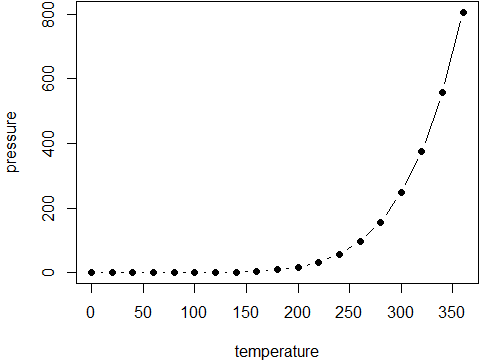
\includegraphics[width=0.8\linewidth]{02-cross-refs_files/figure-latex/nice-fig-1} 

}

\caption{Here is a nice figure!}\label{fig:nice-fig}
\end{figure}

Don't miss Table \ref{tab:nice-tab}.

\begin{Shaded}
\begin{Highlighting}[]
\NormalTok{knitr}\SpecialCharTok{::}\FunctionTok{kable}\NormalTok{(}
  \FunctionTok{head}\NormalTok{(pressure, }\DecValTok{10}\NormalTok{), }\AttributeTok{caption =} \StringTok{\textquotesingle{}Here is a nice table!\textquotesingle{}}\NormalTok{,}
  \AttributeTok{booktabs =} \ConstantTok{TRUE}
\NormalTok{)}
\end{Highlighting}
\end{Shaded}

\begin{table}

\caption{\label{tab:nice-tab}Here is a nice table!}
\centering
\begin{tabular}[t]{rr}
\toprule
temperature & pressure\\
\midrule
0 & 0.0002\\
20 & 0.0012\\
40 & 0.0060\\
60 & 0.0300\\
80 & 0.0900\\
\addlinespace
100 & 0.2700\\
120 & 0.7500\\
140 & 1.8500\\
160 & 4.2000\\
180 & 8.8000\\
\bottomrule
\end{tabular}
\end{table}

\hypertarget{parts}{%
\chapter{Parts}\label{parts}}

You can add parts to organize one or more book chapters together. Parts can be inserted at the top of an .Rmd file, before the first-level chapter heading in that same file.

Add a numbered part: \texttt{\#\ (PART)\ Act\ one\ \{-\}} (followed by \texttt{\#\ A\ chapter})

Add an unnumbered part: \texttt{\#\ (PART\textbackslash{}*)\ Act\ one\ \{-\}} (followed by \texttt{\#\ A\ chapter})

Add an appendix as a special kind of un-numbered part: \texttt{\#\ (APPENDIX)\ Other\ stuff\ \{-\}} (followed by \texttt{\#\ A\ chapter}). Chapters in an appendix are prepended with letters instead of numbers.

\hypertarget{footnotes-and-citations}{%
\chapter{Footnotes and citations}\label{footnotes-and-citations}}

\hypertarget{footnotes}{%
\section{Footnotes}\label{footnotes}}

Footnotes are put inside the square brackets after a caret \texttt{\^{}{[}{]}}. Like this one \footnote{This is a footnote.}.

\hypertarget{citations}{%
\section{Citations}\label{citations}}

Reference items in your bibliography file(s) using \texttt{@key}.

For example, we are using the \textbf{bookdown} package \citep{R-bookdown} (check out the last code chunk in index.Rmd to see how this citation key was added) in this sample book, which was built on top of R Markdown and \textbf{knitr} \citep{xie2015} (this citation was added manually in an external file book.bib).
Note that the \texttt{.bib} files need to be listed in the index.Rmd with the YAML \texttt{bibliography} key.

The \texttt{bs4\_book} theme makes footnotes appear inline when you click on them. In this example book, we added \texttt{csl:\ chicago-fullnote-bibliography.csl} to the \texttt{index.Rmd} YAML, and include the \texttt{.csl} file. To download a new style, we recommend: \url{https://www.zotero.org/styles/}

The RStudio Visual Markdown Editor can also make it easier to insert citations: \url{https://rstudio.github.io/visual-markdown-editing/\#/citations}

\hypertarget{blocks}{%
\chapter{Blocks}\label{blocks}}

\hypertarget{equations}{%
\section{Equations}\label{equations}}

Here is an equation.

\begin{equation} 
  f\left(k\right) = \binom{n}{k} p^k\left(1-p\right)^{n-k}
  \label{eq:binom}
\end{equation}

You may refer to using \texttt{\textbackslash{}@ref(eq:binom)}, like see Equation \eqref{eq:binom}.

\hypertarget{theorems-and-proofs}{%
\section{Theorems and proofs}\label{theorems-and-proofs}}

Labeled theorems can be referenced in text using \texttt{\textbackslash{}@ref(thm:tri)}, for example, check out this smart theorem \ref{thm:tri}.

\begin{theorem}
\protect\hypertarget{thm:tri}{}\label{thm:tri}For a right triangle, if \(c\) denotes the \emph{length} of the hypotenuse
and \(a\) and \(b\) denote the lengths of the \textbf{other} two sides, we have
\[a^2 + b^2 = c^2\]
\end{theorem}

Read more here \url{https://bookdown.org/yihui/bookdown/markdown-extensions-by-bookdown.html}.

\hypertarget{callout-blocks}{%
\section{Callout blocks}\label{callout-blocks}}

The \texttt{bs4\_book} theme also includes special callout blocks, like this \texttt{.rmdnote}.

You can use \textbf{markdown} inside a block.

\begin{Shaded}
\begin{Highlighting}[]
\FunctionTok{head}\NormalTok{(beaver1, }\AttributeTok{n =} \DecValTok{5}\NormalTok{)}
\CommentTok{\#\textgreater{}   day time  temp activ}
\CommentTok{\#\textgreater{} 1 346  840 36.33     0}
\CommentTok{\#\textgreater{} 2 346  850 36.34     0}
\CommentTok{\#\textgreater{} 3 346  900 36.35     0}
\CommentTok{\#\textgreater{} 4 346  910 36.42     0}
\CommentTok{\#\textgreater{} 5 346  920 36.55     0}
\end{Highlighting}
\end{Shaded}

It is up to the user to define the appearance of these blocks for LaTeX output.

You may also use: \texttt{.rmdcaution}, \texttt{.rmdimportant}, \texttt{.rmdtip}, or \texttt{.rmdwarning} as the block name.

The R Markdown Cookbook provides more help on how to use custom blocks to design your own callouts: \url{https://bookdown.org/yihui/rmarkdown-cookbook/custom-blocks.html}

\hypertarget{sharing-your-book}{%
\chapter{Sharing your book}\label{sharing-your-book}}

\hypertarget{publishing}{%
\section{Publishing}\label{publishing}}

HTML books can be published online, see: \url{https://bookdown.org/yihui/bookdown/publishing.html}

\hypertarget{pages}{%
\section{404 pages}\label{pages}}

By default, users will be directed to a 404 page if they try to access a webpage that cannot be found. If you'd like to customize your 404 page instead of using the default, you may add either a \texttt{\_404.Rmd} or \texttt{\_404.md} file to your project root and use code and/or Markdown syntax.

\hypertarget{metadata-for-sharing}{%
\section{Metadata for sharing}\label{metadata-for-sharing}}

Bookdown HTML books will provide HTML metadata for social sharing on platforms like Twitter, Facebook, and LinkedIn, using information you provide in the \texttt{index.Rmd} YAML. To setup, set the \texttt{url} for your book and the path to your \texttt{cover-image} file. Your book's \texttt{title} and \texttt{description} are also used.

This \texttt{bs4\_book} provides enhanced metadata for social sharing, so that each chapter shared will have a unique description, auto-generated based on the content.

Specify your book's source repository on GitHub as the \texttt{repo} in the \texttt{\_output.yml} file, which allows users to view each chapter's source file or suggest an edit. Read more about the features of this output format here:

\url{https://pkgs.rstudio.com/bookdown/reference/bs4_book.html}

Or use:

\begin{Shaded}
\begin{Highlighting}[]
\NormalTok{?bookdown}\SpecialCharTok{::}\NormalTok{bs4\_book}
\end{Highlighting}
\end{Shaded}


  \bibliography{book.bib,packages.bib}

\end{document}
